\chapter{Experimental Setup}
    This chapter explains how we prepared tools and devices for the purpose of experiments for our research work. We have used different third-party tools and frameworks, cloud-services like storages and runtime-machines. Finally, deployment of the trained model to android is discussed here.
        
    \section{Prepare Google Colaboratory}
        We have run the whole experiment in the cloud machines of Google. Their platform ``Colaboratory'' provides access to cloud \acrshort{gpu}s which can accelerate the training process of neural networks.
    
    \section{Preparing the Dataset}
        We have downloaded 380 web-scraped unique images with potholes from the online platform \href{https://kaggle.com}{\itshape{kaggle.com}} and more 285 images we have captured using an android-phone. This is shown in table \ref{tab:img_sources} and visualized in figure \ref{fig:image_sources}.
        
        \begin{table}[ht]
            \centering
            \begin{tabular}{|c|c|c|} \hline
                Image Source &  Number of Images & Percentage \\\hline\hline
                Web-Scraping & 380 & 57.1\% \\\hline
                Camera-Capturing & 285 & 42.9\% \\\hline
            \end{tabular}
            \caption{Sources of Images Collected from}
            \label{tab:img_sources}
        \end{table}
        
        \begin{figure}
            \centering
            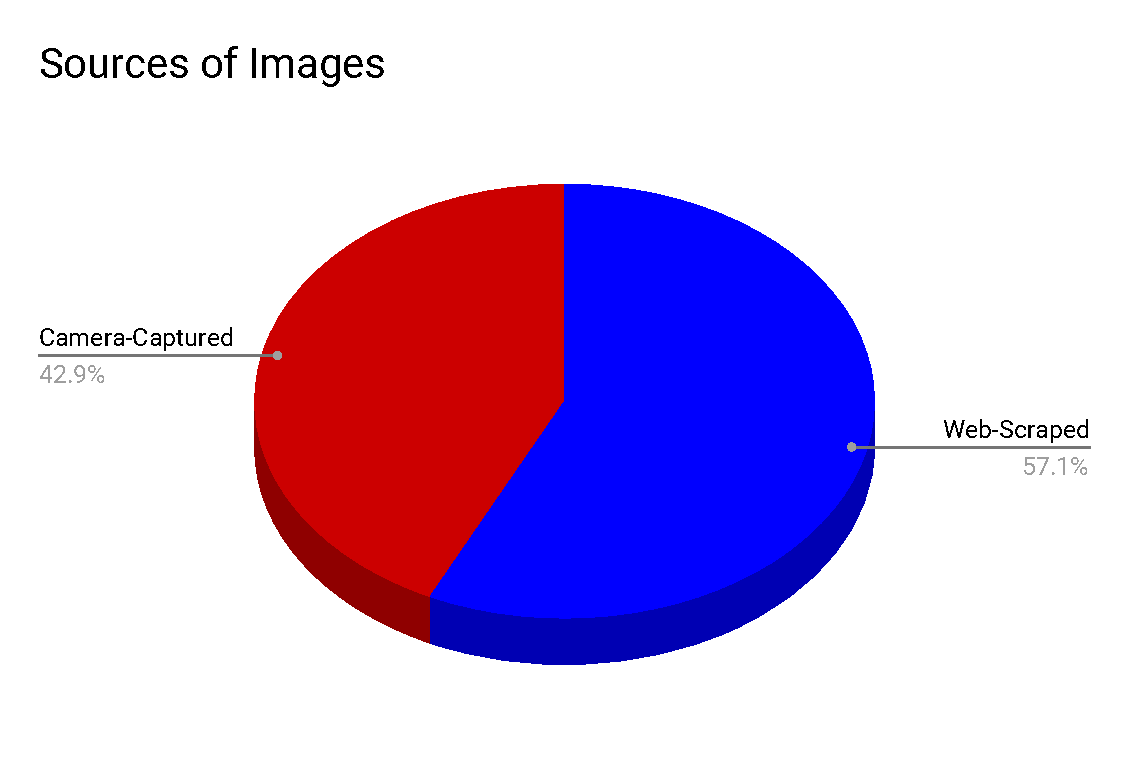
\includegraphics[width=\textwidth]{Sources-of-Images}
            \caption{Sources of Dataset Images}
            \label{fig:image_sources}
        \end{figure}
        
        \clearpage
        \subsection{Annotating the Regions of Interest}
            For detection of objects and things in images, in case of supervised learning, the regions of interest have to be annotated using bounding-boxes or image-segmentation with masking so that the training process can be accomplished.
            
            We have used \gls{labelimg} to select the regions of interest. This tool can generate \acrfull{xml} format file having the annotation details for each image.
        
            \begin{figure}[h]
                \centering
                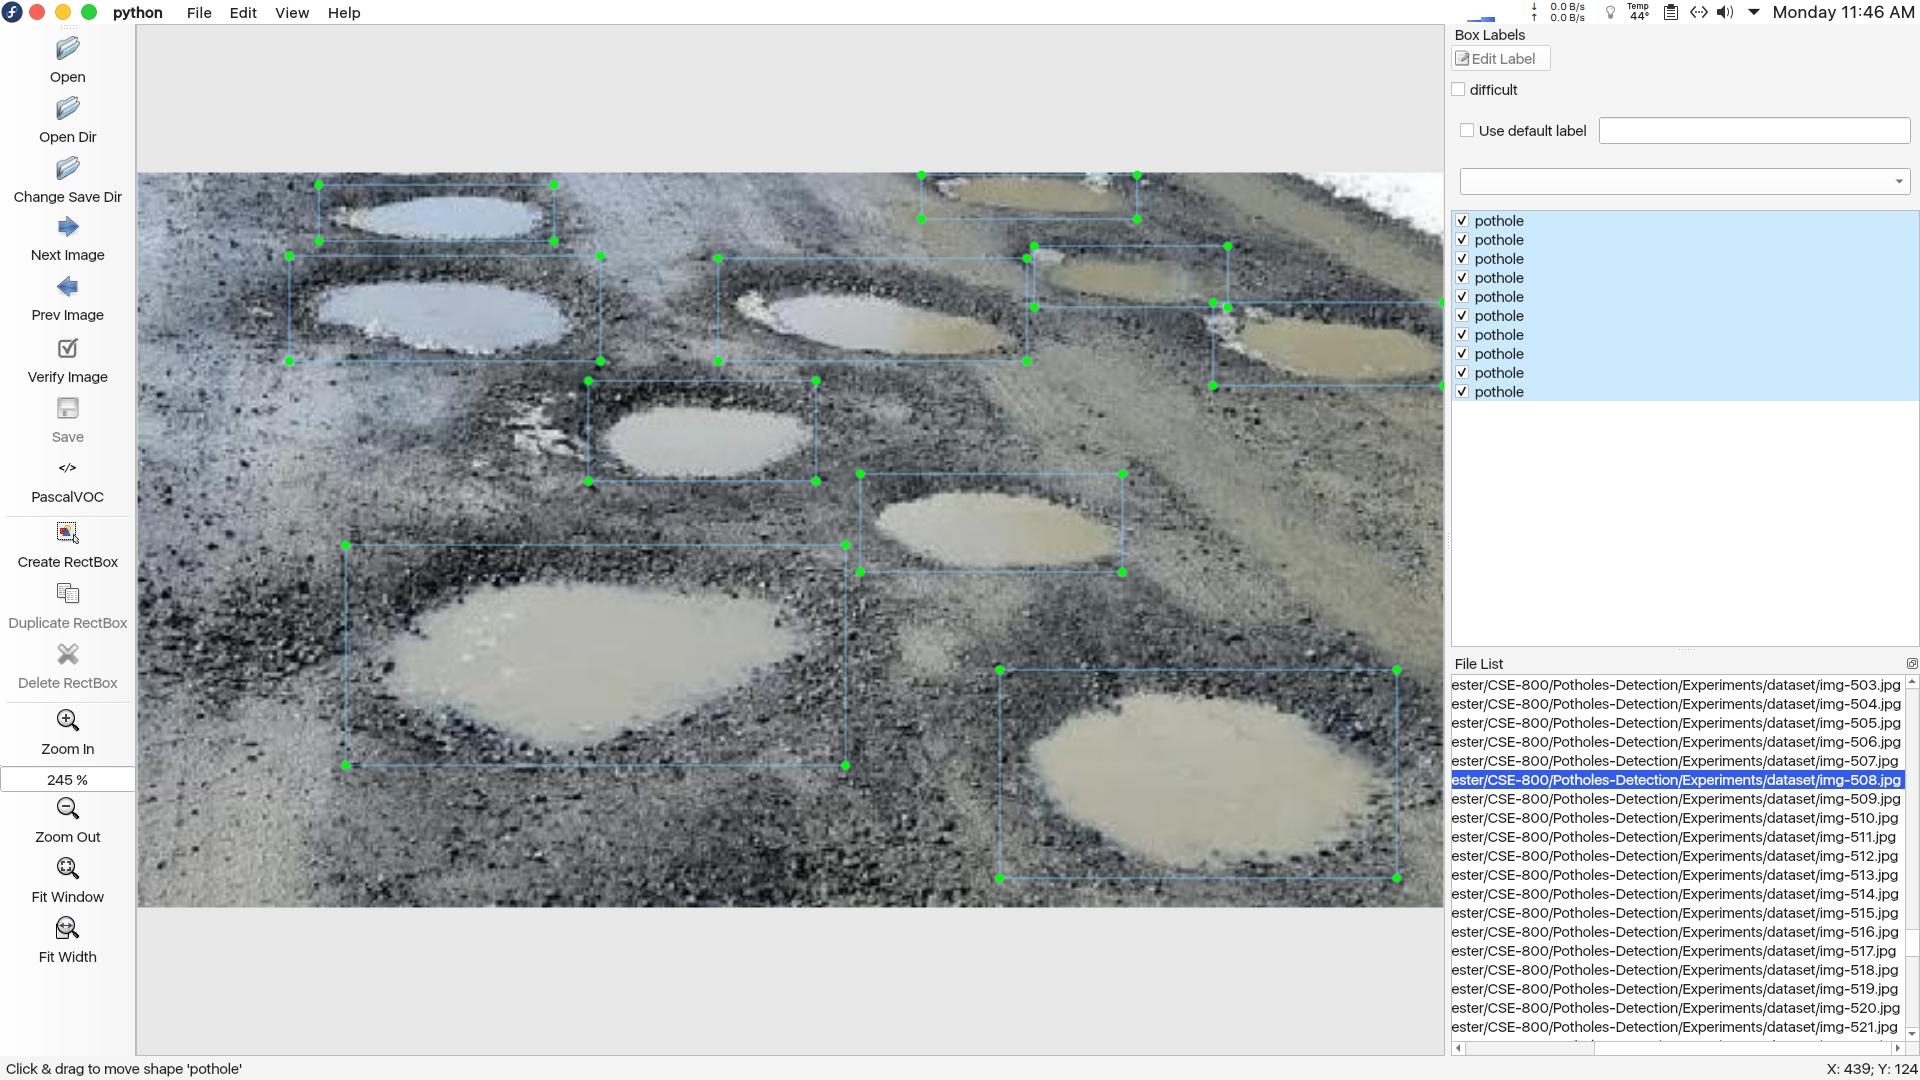
\includegraphics[width=\textwidth]{labelImg}
                \caption{Selecting the Regions of Interest using labelImg}
                \label{fig:labelImg}
            \end{figure}
            
        \subsection{Splitting the Dataset into Train an Validation}
            We have partitioned all the annotated images into two disjoint sets. The set of training data contains 80\% of the total dataset and the set of validation data contains the rest 20\% of total dataset.
            
            \begin{figure}
                \centering
                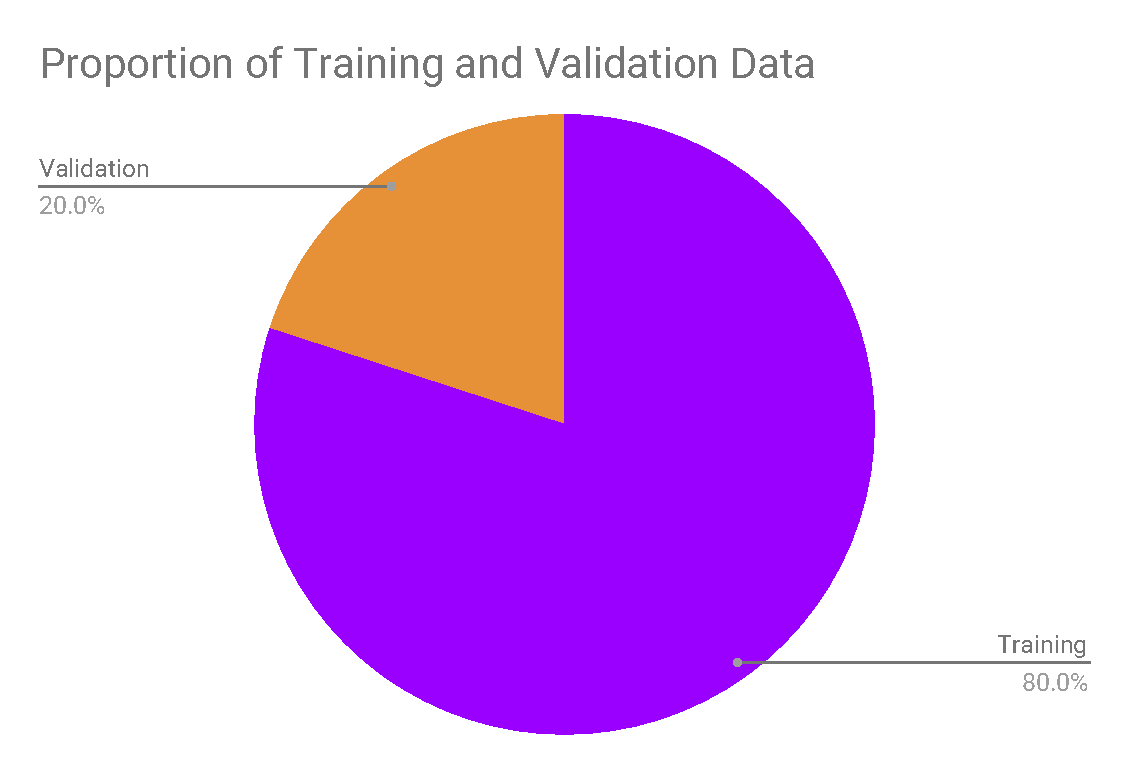
\includegraphics[width=\textwidth]{Proportion-of-Training-and-Validation-Data}
                \caption{Proportion of Training and Validation Data}
                \label{fig:train_test_proportion}
            \end{figure}
        
            \begin{table}
                \centering
                \begin{tabular}{|c|c|c|} \hline
                     &  Number of Images & Percentage \\\hline\hline
                    Training & 532 & 80\% \\\hline
                    Validation & 113 & 20\% \\\hline
                \end{tabular}
                \caption{Proportion of Training and Validation Data}
                \label{tab:train_test_proportion}
            \end{table}
            
            This partitioning was followed by random splitting. The code we used to do this task is given in Appendix \ref{app:ds_split}.
            
        \subsection{Creating tfrecord Files}
            \gls{tensorflow} Object Detection \acrshort{api} uses \gls{tfrecord} file format bundling all the dataset-images along with their regions of interest and class-labels\cite{bisong2019tensorflow}. Therefore, we can feed the tfrecord generated from our dataset. We created two separate tfrecord files--- one for training dataset and another for validation dataset.
            
            Python Code to create \gls{tfrecord} files is given in Appendix \ref{app:mk_tfrecord}.
            
    \section{Preparing a Pre-Trained Model}
        We have followed transfer learning approach\cite{pan2009survey} in this research experiment. So, we required a pre-trained model ready to be used as a base model. There are many pre-trained models trained on different datasets with different metrics. These pre-trained models can be found in \gls{tensorflow}\cite{dillon2017tensorflow} Model Zoo\cite{tf_model_zoo}.
        
        We have used the \acrshort{ssd}\cite{liu2016ssd} \gls{mobilenet}\cite{howard2017mobilenets} V2 pre-trained model which was trained on Microsoft \acrshort{coco} dataset\cite{lin2014microsoft}.
        
        \subsection{Fine-Tune Configuration}
            Every pre-trained model in the \gls{tensorflow} Model Zoo\cite{tf_model_zoo} contains a ``pipeline.config'' file which is used as a configuration file during training and evaluation. We have removed/changed/added several configuration options in that file. Our changes is shown in table \ref{tab:fine_tuned_conf}.
            
            Example of some options the configuration file consists are---
            \begin{itemize}
                \item {Number of classes or labels}
                \item {Activation Functions}
                \item {Prepossessing and Data Augmentation Options}
                \item {Learning Rate and Batch Size}
                \item {Evaluation Methods}
            \end{itemize}
            \begin{table}
                \centering
                \begin{tabular}{|l|l|} \hline 
                     Configuration Option  &  Changed Value \\\hline\hline
                     input\_shape  &  (300, 300, 3) \\\hline
                     num\_classes  &  1 \\\hline
                     image\_resizer  &  keep\_aspect\_ratio\_resizer \\\hline
                     min\_dimension  &  300 \\\hline
                     max\_dimension  &  300 \\\hline
                     pad\_to\_max\_dimension  &  true \\\hline
                     initial\_learning\_rate  &  0.005 \\\hline
                     decay\_steps  &  6000 \\\hline
                     decay\_factor  &  0.85 \\\hline
                     quantization\_delay  &  30000 \\\hline
                \end{tabular}
                \caption{Fine-Tuned Configurations}
                \label{tab:fine_tuned_conf}
            \end{table}
    \section{Prepare TensorFlow Models Repository}
        For the purpose of training as well as validation of our model we reused the existing libraries, packages and codes from the \gls{tensorflow} ``models'' repository. The repository contains almost everything we need for training and evaluation using \gls{tensorflow} \acrshort{api}. The mentioned repository can found in Github\cite{tf_models_repo}.
        
    \section{Launch Tensorboard}
        \gls{tensorboard} is a web-interface which can be used to monitor and visualize the results and performance of the model\cite{manetensorboard}. It is worth mentioning that the \gls{tensorflow} ``models'' repository provides the tools for training and evaluation of models which, if used, saves the parameters, hyper-parameters, scalars and results of model evaluation in ``tfevent'' files\cite{tf_models_repo}. \gls{tensorboard} uses these files and shows the contents graphically in a web-interface\cite{manetensorboard}.
        
    \section{Run Training Process}
        \gls{tensorflow} ``models'' repository provides necessary python code for the whole training process. It also saves the checkpoints of the model in training at a regular interval of time. It starts training from the saved checkpoints if the process is interrupted\cite{tf_models_repo}. It saves the scalar and graphical values i.e. the results of training and evaluation in ``tfevent'' files which can be monitored in \gls{tensorboard}.
        
    \section{Run Evaluation Process}
        After the training process ends, we can run the evaluation on the validation dataset. \gls{tensorflow} ``models'' repository provides the tools for the evaluation process too. The evaluation is triggered by the training tool automatically whenever it saves a checkpoint of the model\cite{tf_models_repo}. This helps to monitor the performance of the model at different level of training steps and epochs.
            
    \begin{figure}[h]
        \centering
        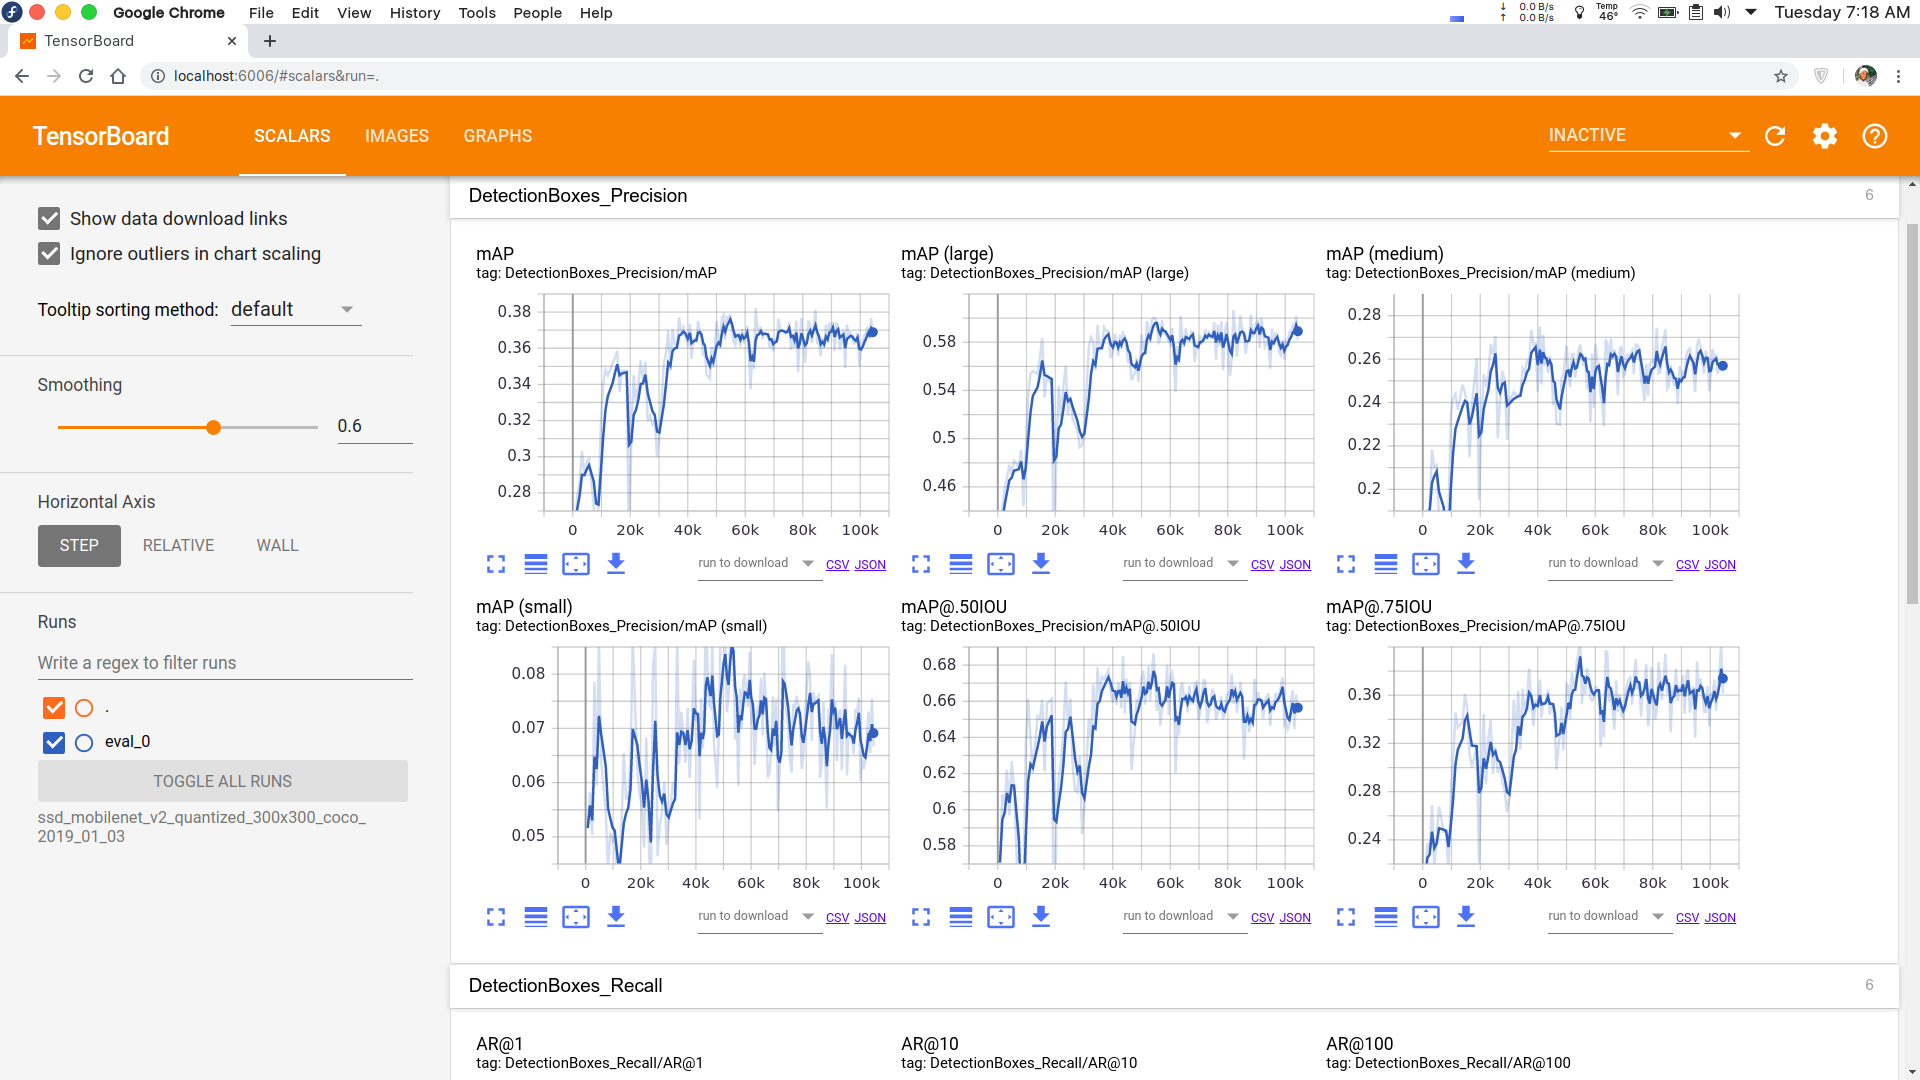
\includegraphics[height=\dimexpr\pagegoal-\pagetotal-\baselineskip\relax,width=\textwidth,keepaspectratio]{tensorboard}
        \caption{Visualizing and Monitoring the Model and Progress in Tensorboard}
        \label{fig:tb_ui}
    \end{figure}
